\section{$N^2$ Chart}
The $N^2$ chart shows the interfaces between the different functions of the system. The chart could be found in figure \ref{fig:n2chart} on page \pageref{fig:n2chart}. The functions are in the dark grey boxes, while the interactions are shown by the dotted boxes and move clockwise. The system is split up in the emitter satellite, a receiver satellite and the ground segment, denoted by the large bold boxes. Outside of these boxes is the outside world, e.g. the Sun and customers. The starred interactions dependent on the level of communication centralisation.

\begin{figure}
\centering
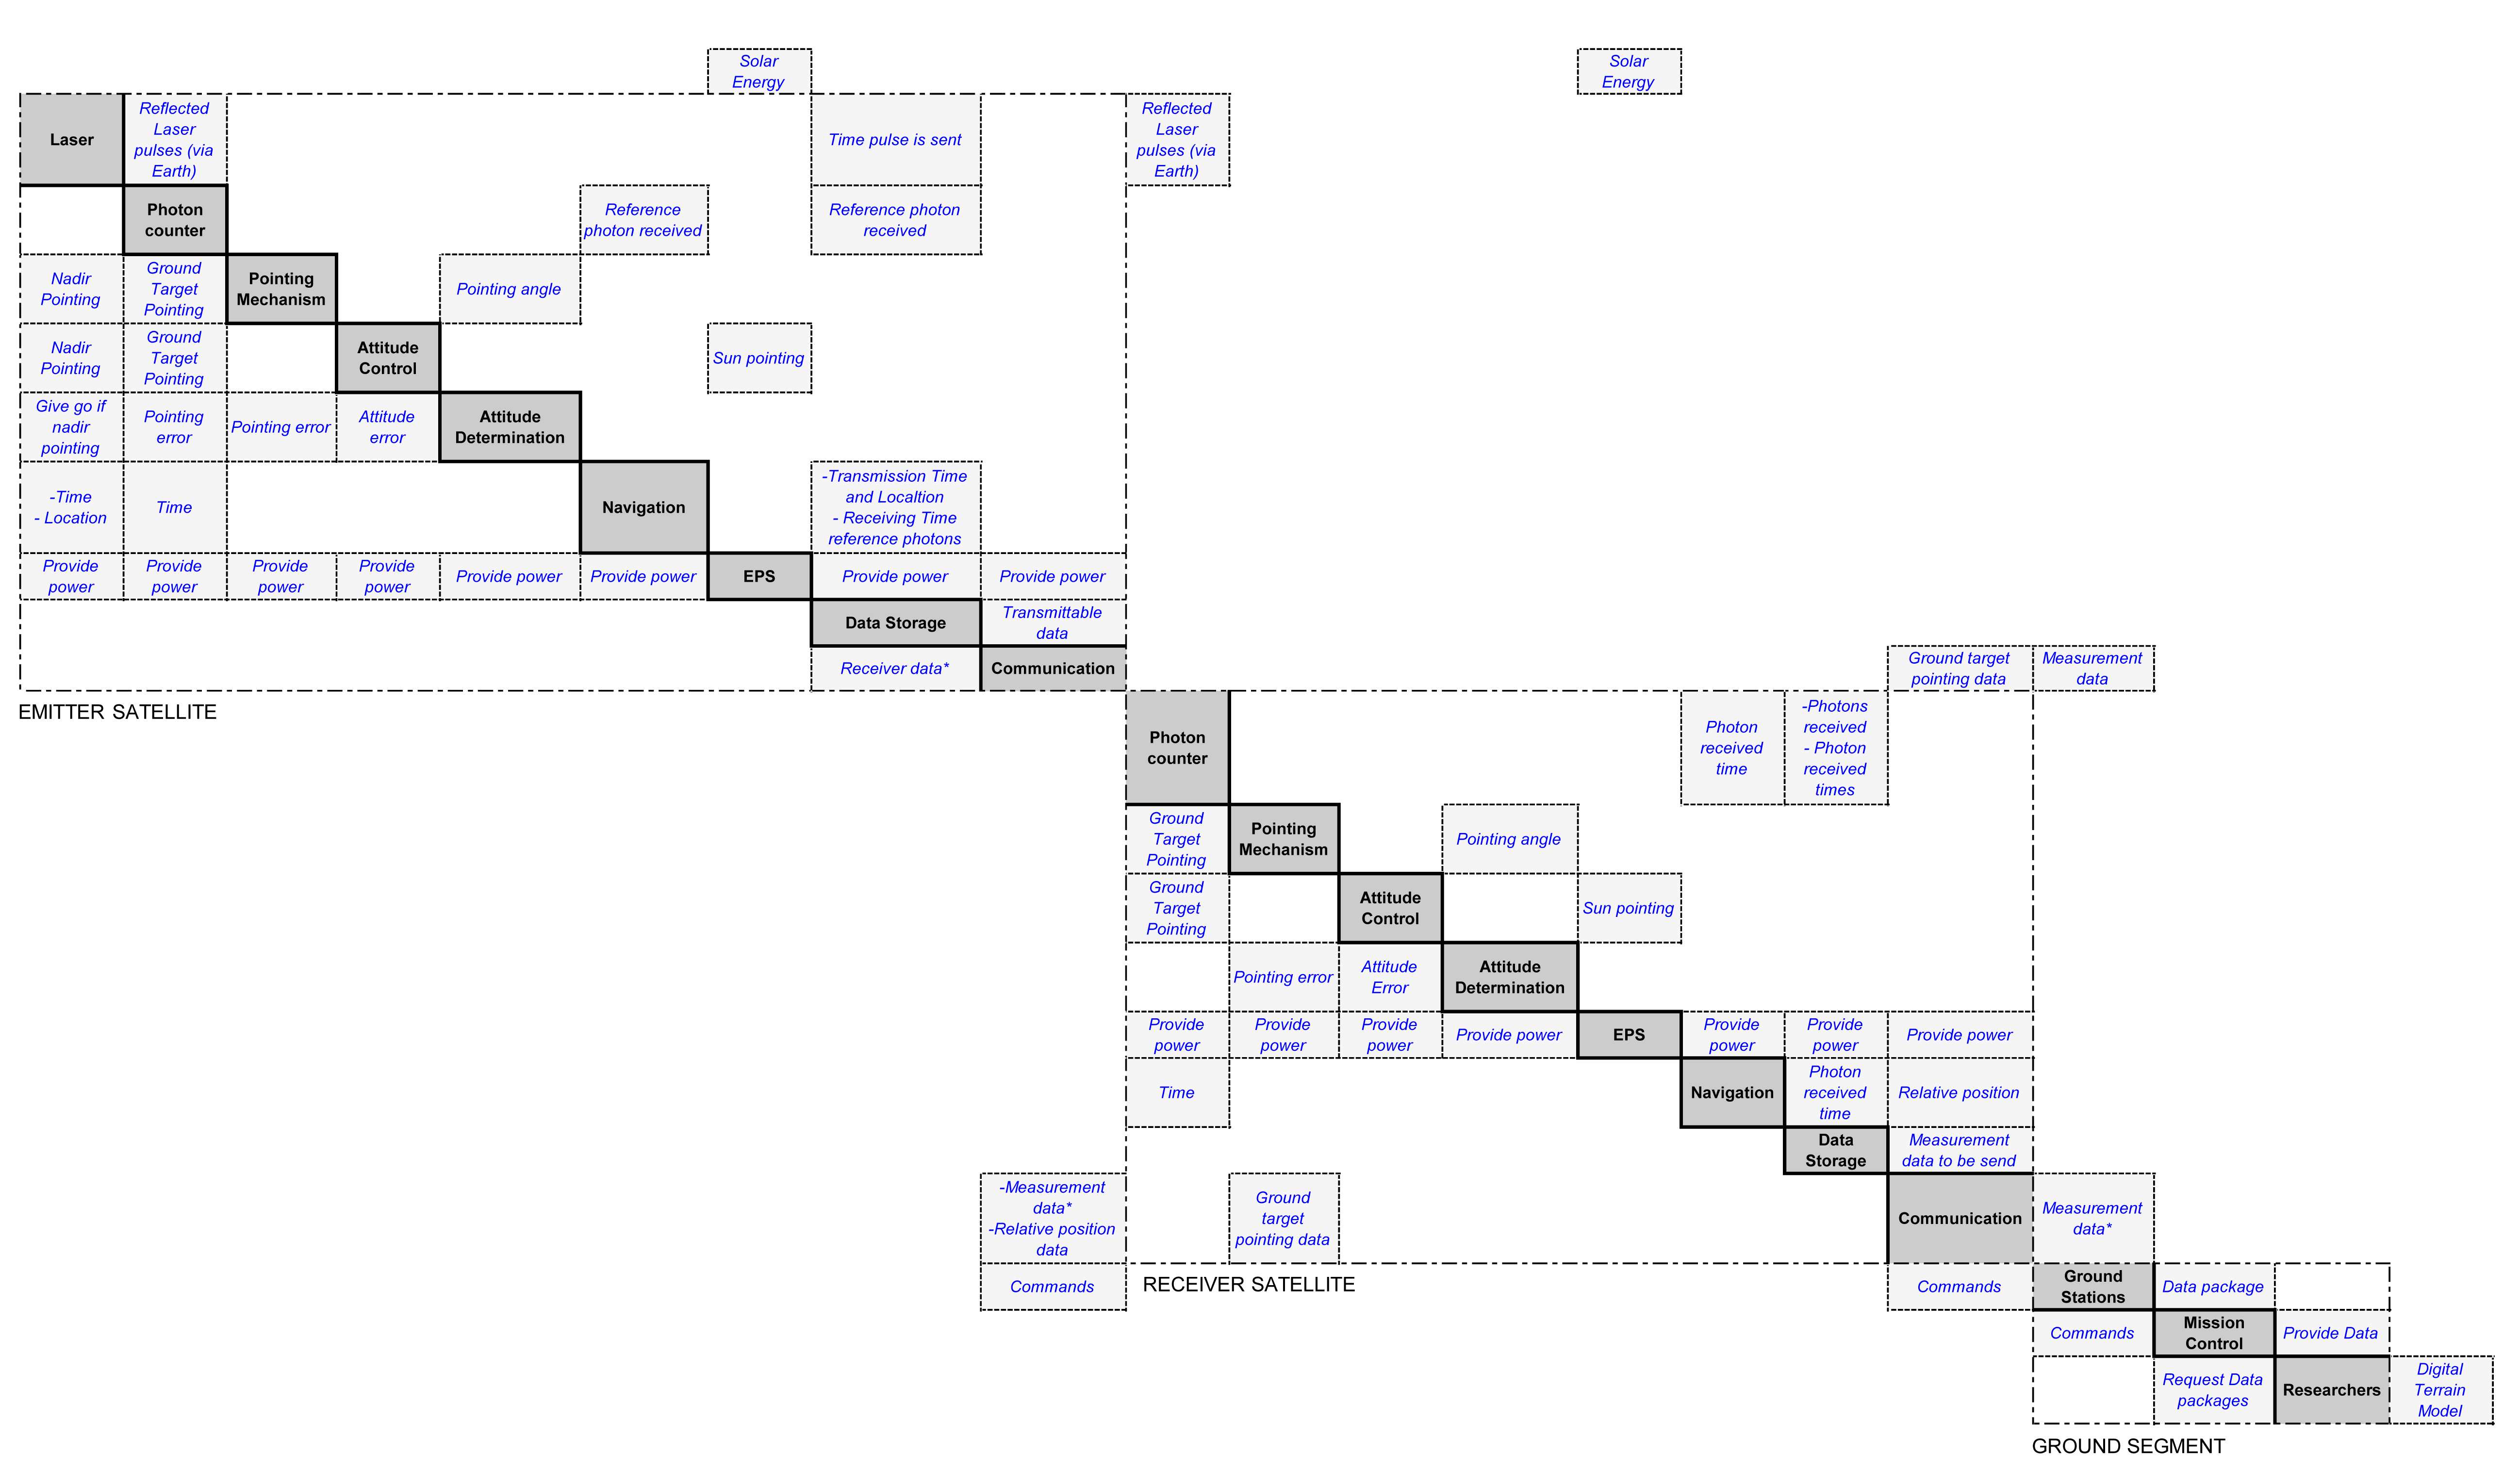
\includegraphics[angle = 90, width = 0.7\textwidth, bb= 0 0 3421px 1861px]{img/N2chart_wo.png} 
\caption{$N^2$ chart of the Laser Swarm mission}
\label{fig:n2chart}
\end{figure}